\documentclass[border=10pt]{standalone}
\usepackage{pgfplots}
\pgfplotsset{compat=1.18}
\usepgfplotslibrary{colormaps}

\begin{document}
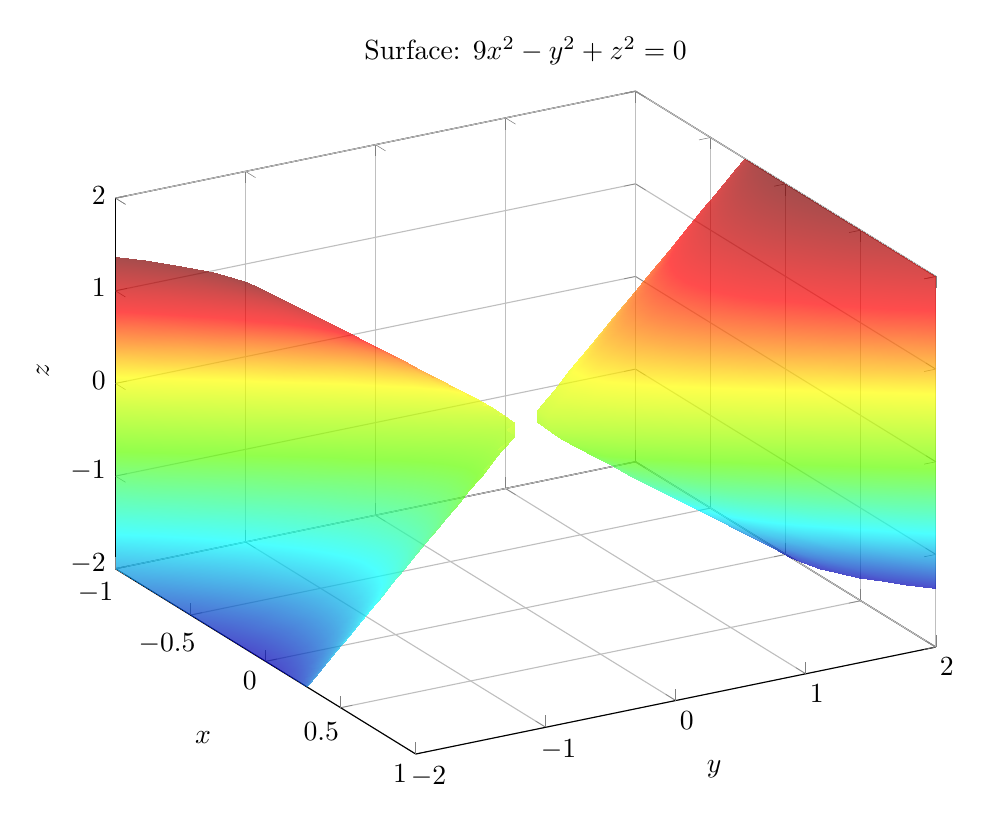
\begin{tikzpicture}
\begin{axis}[
    view={60}{30},
    xlabel={$x$},
    ylabel={$y$},
    zlabel={$z$},
    title={Surface: $9x^2 - y^2 + z^2 = 0$},
    domain=-1:1,
    y domain=-2:2,
    samples=30,
    samples y=30,
    colormap/bluered,
    grid=major,
    width=12cm,
    height=10cm,
    zmin=-2,
    zmax=2,
    xmin=-1,
    xmax=1,
    ymin=-2,
    ymax=2
]
% Upper nappe: y = sqrt(9x^2 + z^2)
\addplot3[surf, shader=interp, opacity=0.7, blue] 
    ({x}, {sqrt(9*x^2 + y^2)}, {y});
% Lower nappe: y = -sqrt(9x^2 + z^2)
\addplot3[surf, shader=interp, opacity=0.7, red] 
    ({x}, {-sqrt(9*x^2 + y^2)}, {y});
\end{axis}
\end{tikzpicture}
\end{document}